\documentclass[tikz,border=3pt]{standalone}
\usepackage[T1]{fontenc}
\usepackage{helvet}
\renewcommand{\familydefault}{\sfdefault}
\usepackage{setspace}
\usetikzlibrary{positioning,arrows.meta,shapes.geometric}

\begin{document}
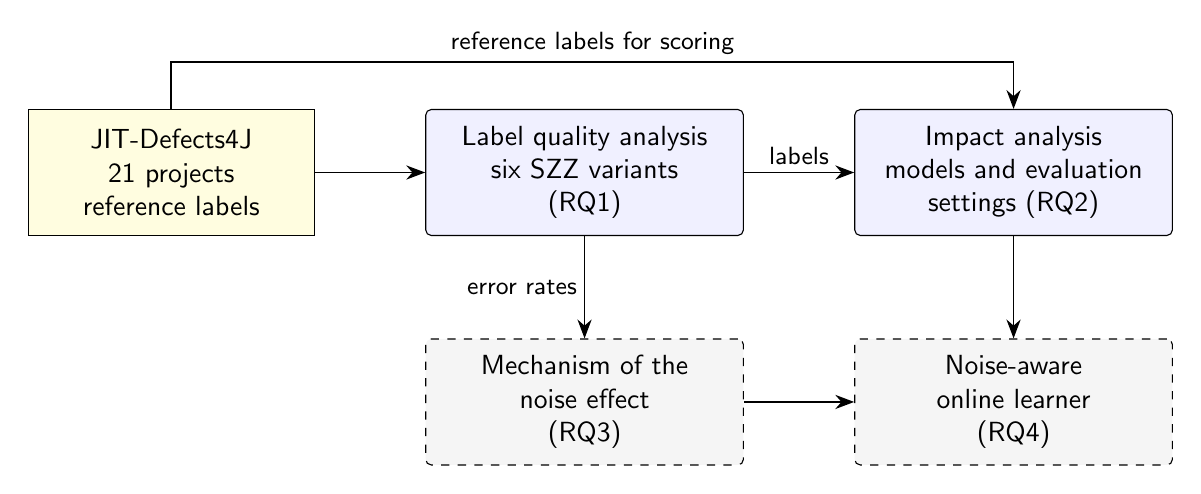
\begin{tikzpicture}[node distance=7mm and 14mm,
  box/.style={draw, rounded corners=2pt, align=center, text width=38mm, minimum height=16mm, fill=blue!6},
  plan/.style={box, dashed, fill=gray!8},
  data/.style={draw, align=center, text width=34mm, minimum height=16mm, fill=yellow!12},
  arr/.style={-{Stealth[length=2.4mm]}, semithick},
  lab/.style={font=\small, fill=white, inner sep=1.5pt}]
\node[data] (ref) {JIT-Defects4J\\21 projects\\reference labels};
\node[box, right=of ref] (s1) {Label quality analysis\\six SZZ variants\\(RQ1)};
\node[box, right=of s1] (s2) {Impact analysis\\models and evaluation\\settings (RQ2)};
\node[plan, below=13mm of s1] (s3) {Mechanism of the\\noise effect\\(RQ3)};
\node[plan, below=13mm of s2] (s4) {Noise-aware\\online learner\\(RQ4)};
\draw[arr] (ref) -- (s1);
\draw[arr] (s1) -- node[lab, above=1pt] {labels} (s2);
\draw[arr] (s1) -- node[lab, left=1pt] {error rates} (s3);
\draw[arr] (s2) -- (s4);
\draw[arr] (s3) -- (s4);
\draw[arr] (ref.north) -- ++(0,6mm) -| node[lab, pos=0.25, above=1pt] {reference labels for scoring} (s2.north);
\end{tikzpicture}
\end{document}
